
\section{Evaluation}

Details of our experiments follow, with a concluding discussion section.

\begin{table*}
\caption{
    Mean APs (or accuracies, where noted) on three datasets for the considered single-channel features and their second-stage combination.
    As some features were clearly dominated by others on the AVA dataset, only the better features were evaluated on larger datasets.
}
\label{tab:mean_aps}
\centering
\small{
\begin{tabular}{lrrrrrrrrr}
\toprule
{} &  Late-fusion &  DeCAF$_5$ &  DeCAF$_6$ &  MC-bit &  Tuned DC$_6$ &  L*a*b* Hist &  GIST &  Saliency &  random \\
\midrule
AVA Rating (acc.) &                  - &    0.779 &    0.686 &   0.843 &               0.720 &             0.574 & 0.558 &                 0.539 &   0.500 \\
AVA Style             &                  0.604 &    0.427 &    0.577 &   0.529 &               0.552 &             0.291 & 0.220 &                 0.149 &   0.127 \\
Flickr                &                  0.419 &    0.314 &    0.391 &   0.360 &               0.396 &                 - &     - &                     - &   0.066 \\
Wikipaintings         &                  0.476 &        - &    0.356 &   0.443 &               0.356 &                 - &     - &                     - &   0.043 \\
\bottomrule
\end{tabular}
}
\end{table*}

\subsection{AVA Style}

We evaluate classification of aesthetic rating and of 14 different photographic style labels on the 14,000 images of the AVA dataset that have such labels.
For the style labels, the publishers of the dataset provide a train/test split, where training images have only one label, but test images may have more than one label \cite{Murray-CVPR-2012}.
Although the provided test split has an uneven class distribution, we found that to compare with the reported results, a class-balanced set is needed.

Consequently, we adhere to the provided split but compute evaluation metrics on a random class-balanced subset of the test data.
We use class-balanced data for evaluation in all following experiments.

\vspace{-.5em}
\paragraph{Metrics.}
Following the established approach, aesthetic rating is classified in a binary prediction task of being below or above the mean.
On this task, we report the accuracy of our predictions.

For multi-class prediction of the style labels, we report the confusion matrix of most confident classifications for each image, top-K accuracies (useful to see when the dataset has easily confused labels), and per-class Average Precision (AP): area under the Precision vs.~Recall curve.
% TODO: uncomment for camera ready
% For space constraints, we do not include all of these plots and tables in the main body of the paper, but provide them in entirety in the supplemental materials.

\vspace{-.5em}
\paragraph{Results.}
For all features, AP scores for the AVA Style dataset are shown in~\autoref{fig:ava_style_results}.
The mean AP scores and the aesthetic rating accuracy are given in the overall results table~\autoref{tab:mean_aps}.

For aesthetic rating performance, the best single feature is the MC-bit feature, obtaining 0.843 accuracy.
Previous work did not report accuracy on this subset of the data, but their best reported accuracy on the test set of the full AVA data is 0.68 \cite{Murray-CVPR-2012}.
For style classification, the best single feature is the DeCAF$_6$ convolution network feature, obtaining 0.577 mean AP.
Feature fusion improves the result to 0.604 mean AP; both results beat the previous state-of-the-art of 0.538 mean AP \cite{Murray-CVPR-2012}.

In all metrics, the DeCAF and MC-bit features significantly outperform the more low-level features.
Accordingly, we do not evaluate the low-level features on the larger Flickr and Wikipaintings datasets.

\begin{figure}
\centering
\includegraphics[width=\linewidth]{../arxiv/figures/evaluation/ava_style_ap_barplot.pdf}
\caption{APs on the AVA Style dataset. }
\label{fig:ava_style_results}
\end{figure}

\subsection{Flickr Style}

\begin{figure}
\centering
\includegraphics[width=\linewidth]{../arxiv/figures/evaluation/flickr_ap_barplot.pdf}
\caption{APs on the Flickr dataset.}
\label{fig:flickr_results}
\end{figure}

Following the same evaluation setup and metrics as above, we learn and predict style labels on the 53,000 images labeled with 18 different visual styles of our new Flickr Style dataset, using 20\% of the data for testing, and another 20\% for parameter tuning validation.
Results are presented in Figures~\ref{fig:flickr_results} and \ref{fig:top_k}, and in~\autoref{tab:mean_aps}.

The best single-channel feature is again DeCAF$_6$ with 0.396 mean AP; feature fusion obtains 0.419 mean AP.
Surprisingly, fine-tuning the DeCAF convolution net with images from our datasets did not increase performance.

\vspace{-.5em}
\paragraph{Content correlations.}
We plot the confusion matrix of this single-label dataset in~\autoref{fig:flickr_confusion}.
As expected, there are points of understandable confusion: Depth of Field vs. Macro, Romantic vs. Pastel, Vintage vs. Melancholy.
There are also surprising sources of mistakes: Macro vs. Bright/Energetic, for example.

To explain this particular confusion, we observed that lots of Macro photos contain bright flowers, insects, or birds, often against vibrant greenery.
Here, at least, the content of the image dominates its style label.

To explore further content-style correlations, we plot the outputs of PASCAL object class classifiers (one of our features) on the Flickr dataset in~\autoref{fig:content_correlation}.
We can observe that some styles have strong correlations to content (e.g. ``Hazy'' occurs with ``vehicle'', ``HDR'' doesn't occur with ``cat'').
To further enable our linear classifier to take advantage of such correlations, we take an outer product of our content classifier features with the second-stage late fusion features (``Late-fusion $\times$ Content'' in all results figures).

\begin{figure}[h]
\centering
\includegraphics[width=1\linewidth]{../arxiv/figures/evaluation/flickr_conf.pdf}
\caption{
    Confusion matrix of our best classifier (\mbox{Late-fusion $\times$ Content}) on the Flickr dataset.
}
\label{fig:flickr_confusion}
\end{figure}

\begin{figure}[h]
\centering
\includegraphics[width=.9\linewidth]{../arxiv/figures/content_correlation/pascal_on_flickr.pdf}
\caption{
    Correlation of PASCAL content classifers (columns) against ground truth Flickr style labels (rows).
}
\label{fig:content_correlation}
\end{figure}

\subsection{Wikipaintings}

With the same setup and features as in the Flickr experiments, we evaluate 85,000 images labeled with 22 different art styles.
The results are given in Figures~\ref{fig:wikipaintings_style_results} and \ref{fig:top_k}, and in~\autoref{tab:mean_aps}.
The best single-channel feature is MC-bit with 0.444 mean AP; feature fusion obtains 0.476 mean AP.
As with Flickr, fine-tuning the convolutional net feature did not increase its performance on this dataset.

\begin{figure}
\centering
\includegraphics[width=\linewidth]{../arxiv/figures/evaluation/wikipaintings_ap_barplot.pdf}
\caption{APs on the Wikipaintings dataset.}
\label{fig:wikipaintings_style_results}
\end{figure}

\begin{figure}
\centering
\includegraphics[width=.45\linewidth]{../arxiv/figures/evaluation/flickr_top_k.pdf}
\includegraphics[width=.45\linewidth]{../arxiv/figures/evaluation/wikipaintings_top_k.pdf}
\caption{Top-K accuracies for the Flickr and Wikipaintings datasets, respectively. }
\label{fig:top_k}
\end{figure}

%!TEX root = paper/paper.tex
\subsection{Application: Style-Based Image Search}

\newcommand{\fgap}{.6in}
\begin{figure}[h!]
\centering
\begin{tabular}{m{.02in}|m{\fgap} m{\fgap} m{\fgap} m{\fgap} m{\fgap}}
    \begin{turn}{90}\footnotesize{Minimal}\end{turn} &
    \includegraphics[width=.75in]{../../figures/flickr_on_flickr/pred_style_Minimal/w/0.jpg} &
    \includegraphics[width=.75in]{../../figures/flickr_on_flickr/pred_style_Minimal/w/1.jpg} &
    \includegraphics[width=.75in]{../../figures/flickr_on_flickr/pred_style_Minimal/w/2.jpg} &
    \includegraphics[width=.75in]{../../figures/flickr_on_flickr/pred_style_Minimal/w/3.jpg} &
    \includegraphics[width=.75in]{../../figures/flickr_on_flickr/pred_style_Minimal/w/4.jpg} \\
    \begin{turn}{90}\footnotesize{Melancholy}\end{turn} &
    \includegraphics[width=.75in]{../../figures/flickr_on_flickr/pred_style_Melancholy/w/0.jpg} &
    \includegraphics[width=.75in]{../../figures/flickr_on_flickr/pred_style_Melancholy/w/1.jpg} &
    \includegraphics[width=.75in]{../../figures/flickr_on_flickr/pred_style_Melancholy/w/2.jpg} &
    \includegraphics[width=.75in]{../../figures/flickr_on_flickr/pred_style_Melancholy/w/3.jpg} &
    \includegraphics[width=.75in]{../../figures/flickr_on_flickr/pred_style_Melancholy/w/4.jpg} \\
    \begin{turn}{90}\footnotesize{HDR}\end{turn} &
    \includegraphics[width=.75in]{../../figures/flickr_on_flickr/pred_style_HDR/w/0.jpg} &
    \includegraphics[width=.75in]{../../figures/flickr_on_flickr/pred_style_HDR/w/1.jpg} &
    \includegraphics[width=.75in]{../../figures/flickr_on_flickr/pred_style_HDR/w/2.jpg} &
    \includegraphics[width=.75in]{../../figures/flickr_on_flickr/pred_style_HDR/w/3.jpg} &
    \includegraphics[width=.75in]{../../figures/flickr_on_flickr/pred_style_HDR/w/4.jpg} \\
    \begin{turn}{90}\footnotesize{Vintage}\end{turn} &
    \includegraphics[width=.75in]{../../figures/flickr_on_flickr/pred_style_Vintage/w/0.jpg} &
    \includegraphics[width=.75in]{../../figures/flickr_on_flickr/pred_style_Vintage/w/1.jpg} &
    \includegraphics[width=.75in]{../../figures/flickr_on_flickr/pred_style_Vintage/w/2.jpg} &
    \includegraphics[width=.75in]{../../figures/flickr_on_flickr/pred_style_Vintage/w/3.jpg} &
    \includegraphics[width=.75in]{../../figures/flickr_on_flickr/pred_style_Vintage/w/4.jpg} \\
\end{tabular}
\vspace{1em}
\caption{
    Top five most-confident positive predictions on the Flickr Style test set, for a few different styles.
    See Figures 1-3 of the Supplemental Material for more results.
}\label{fig:flickr_on_flickr}
\end{figure}


Style classifiers learned on our datasets can be used toward novel goals.
For example, sources of stock photography or design inspiration may be better navigated with a vocabulary of style.
Currently, companies expend labor to manually annotate stock photography with such labels.
With our approach, any image collection can be searchable and rankable by style.

To demonstrate, we apply our Flickr-learned style classifiers to a new dataset of 80K images gathered on Pinterest (also available with our code release); some results are shown in \autoref{fig:flickr_on_pinterest}.
Interestingly, styles learned from photographs can be used to order paintings, and styles learned from paintings can be used to order photographs, as illustrated in \autoref{fig:photo_painting}.

\begin{figure*}[ht]
\centering
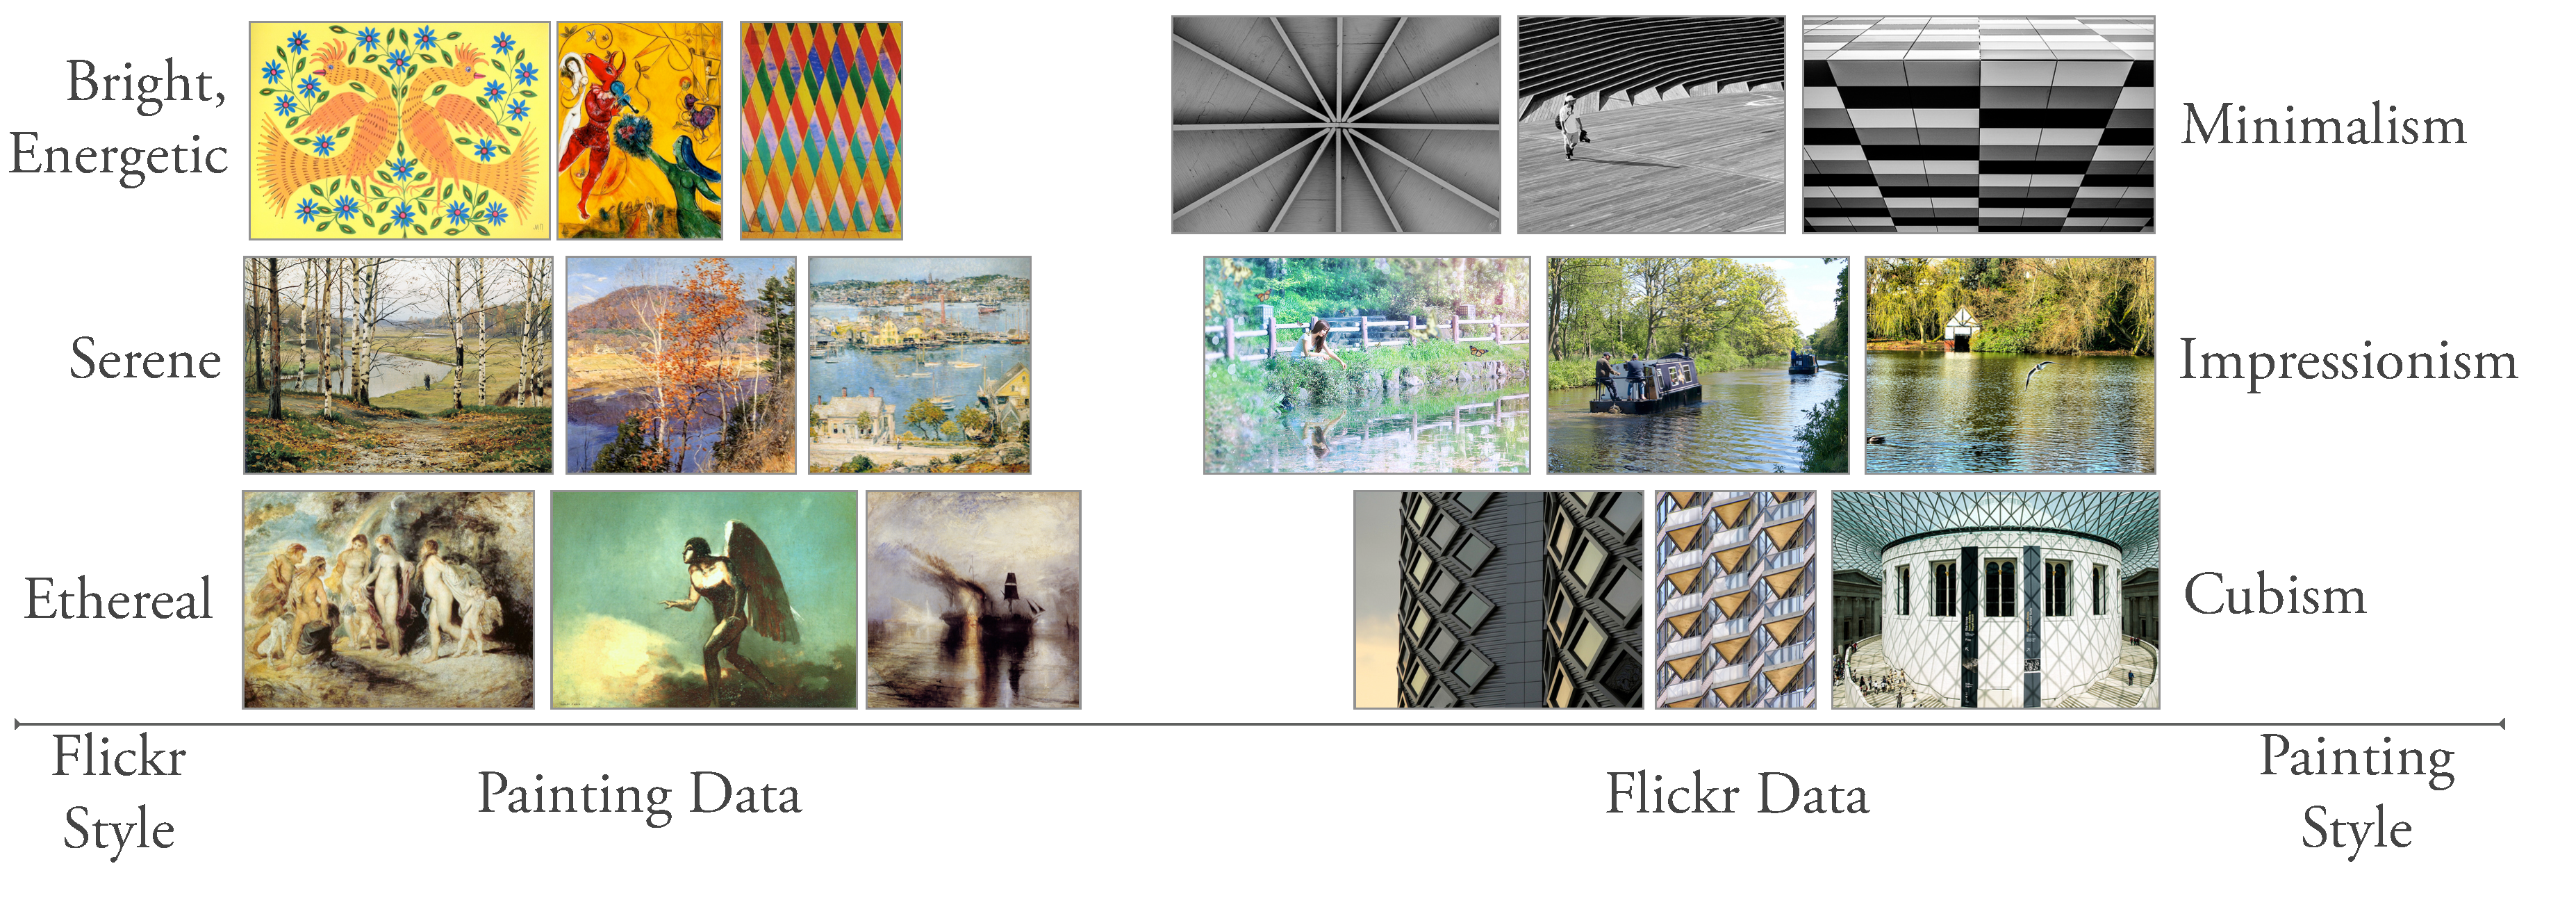
\includegraphics[width=.95\linewidth]{../../figures/style_by_style.pdf}
\vspace{-1ex}
\caption{
    Cross-dataset style.
    On the left are shown top scorers from the Wikipaintings set, for styles learned on the Flickr set.
    On the right, Flickr photographs are accordingly sorted by Painting style.
    (Figure best viewed in color.)
}
\label{fig:photo_painting}
\end{figure*}

\newcommand{\dgap}{.42in}
\begin{figure}
\begin{subfigure}[t]{0.48\linewidth}
    \begin{tabular}{m{.02in}|m{\dgap} m{\dgap} m{\dgap}}
    \begin{turn}{90}\small{Bright}\end{turn} &
    \includegraphics[width=.53in]{../../figures/flickr_on_pinterest/dress/pred_style_Bright/h/0.jpg} &
    \includegraphics[width=.53in]{../../figures/flickr_on_pinterest/dress/pred_style_Bright/h/1.jpg} &
    \includegraphics[width=.53in]{../../figures/flickr_on_pinterest/dress/pred_style_Bright/h/2.jpg} \\ \\
    \begin{turn}{90}\small{Pastel}\end{turn} &
    \includegraphics[width=.53in]{../../figures/flickr_on_pinterest/dress/pred_style_Pastel/h/0.jpg} &
    \includegraphics[width=.53in]{../../figures/flickr_on_pinterest/dress/pred_style_Pastel/h/1.jpg} &
    \includegraphics[width=.53in]{../../figures/flickr_on_pinterest/dress/pred_style_Pastel/h/2.jpg} \\ \\
    \begin{turn}{90}\small{Ethereal}\end{turn} &
    \includegraphics[width=.53in]{../../figures/flickr_on_pinterest/dress/pred_style_Ethereal/h/0.jpg} &
    \includegraphics[width=.53in]{../../figures/flickr_on_pinterest/dress/pred_style_Ethereal/h/1.jpg} &
    \includegraphics[width=.53in]{../../figures/flickr_on_pinterest/dress/pred_style_Ethereal/h/2.jpg} \\ \\
    \begin{turn}{90}\small{Noir}\end{turn} &
    \includegraphics[width=.53in]{../../figures/flickr_on_pinterest/dress/pred_style_Noir/h/0.jpg} &
    \includegraphics[width=.53in]{../../figures/flickr_on_pinterest/dress/pred_style_Noir/h/1.jpg} &
    \includegraphics[width=.53in]{../../figures/flickr_on_pinterest/dress/pred_style_Noir/h/2.jpg} \\ \\
    \begin{turn}{90}\small{Vintage}\end{turn} &
    \includegraphics[width=.53in]{../../figures/flickr_on_pinterest/flower/pred_style_Vintage/h/0.jpg} &
    \includegraphics[width=.53in]{../../figures/flickr_on_pinterest/flower/pred_style_Vintage/h/2.jpg} &
    \includegraphics[width=.53in]{../../figures/flickr_on_pinterest/flower/pred_style_Vintage/h/3.jpg} \\
    \end{tabular}
    \caption{Query: ``dress''.}
\end{subfigure}\hfill%
\begin{subfigure}[t]{0.48\linewidth}
    \begin{tabular}{m{.02in}|m{\dgap} m{\dgap} m{\dgap}}
    \begin{turn}{90}\small{DoF}\end{turn} &
    \includegraphics[width=.53in]{../../figures/flickr_on_pinterest/flower/pred_style_Depth_of_Field/h/1.jpg} &
    \includegraphics[width=.53in]{../../figures/flickr_on_pinterest/flower/pred_style_Depth_of_Field/h/3.jpg} &
    \includegraphics[width=.53in]{../../figures/flickr_on_pinterest/flower/pred_style_Depth_of_Field/h/4.jpg} \\ \\
    \begin{turn}{90}\small{Romantic}\end{turn} &
    \includegraphics[width=.53in]{../../figures/flickr_on_pinterest/flower/pred_style_Romantic/h/0.jpg} &
    \includegraphics[width=.53in]{../../figures/flickr_on_pinterest/flower/pred_style_Romantic/h/1.jpg} &
    \includegraphics[width=.53in]{../../figures/flickr_on_pinterest/flower/pred_style_Romantic/h/3.jpg} \\ \\
    \begin{turn}{90}\small{Sunny}\end{turn} &
    \includegraphics[width=.53in]{../../figures/flickr_on_pinterest/flower/pred_style_Sunny/h/0.jpg} &
    \includegraphics[width=.53in]{../../figures/flickr_on_pinterest/flower/pred_style_Sunny/h/1.jpg} &
    \includegraphics[width=.53in]{../../figures/flickr_on_pinterest/flower/pred_style_Sunny/h/2.jpg} \\ \\
    \begin{turn}{90}\small{Geometric}\end{turn} &
    \includegraphics[width=.53in]{../../figures/flickr_on_pinterest/flower/pred_style_Geometric_Composition/h/0.jpg} &
    \includegraphics[width=.53in]{../../figures/flickr_on_pinterest/flower/pred_style_Geometric_Composition/h/1.jpg} &
    \includegraphics[width=.53in]{../../figures/flickr_on_pinterest/flower/pred_style_Geometric_Composition/h/4.jpg} \\ \\
    \begin{turn}{90}\small{Serene}\end{turn} &
    \includegraphics[width=.53in]{../../figures/flickr_on_pinterest/flower/pred_style_Serene/h/0.jpg} &
    \includegraphics[width=.53in]{../../figures/flickr_on_pinterest/flower/pred_style_Serene/h/2.jpg} &
    \includegraphics[width=.53in]{../../figures/flickr_on_pinterest/flower/pred_style_Serene/h/3.jpg} \\
    \end{tabular}
    \caption{Query: ``flower''.}
\end{subfigure}
\\
\caption{
    Example of filtering image search results by style.
    Our Flickr Style classifiers are applied to images found on Pinterest.
    The images are searched by the text contents of their captions, then filtered by the response of the style classifiers.
    Here we show three out of top five results for different query/style combinations.
}\label{fig:flickr_on_pinterest}
\end{figure}


